%************************************************
\chapter{Un modèle morphologique de scènes sonores environnementales}\label{ch:psycho_model} % $\mathbb{ZNR}$
%************************************************

\section{Motivations}

\subsection{Analyse sensorielle}

\gl{G0: étude de la contribution des sources sonores} \\

\gl{G1: from WAC2015} Some generative systems have already been proposed to generate sound environments \citep{misra2006new,misra2007musical,valle2009framework,finney2010soundscape,schirosa2010system}. Those methods are mostly designed to be used in the sonification of virtual sound environments \citep{valle2009framework,finney2010soundscape}. They may be seen as semi-autonomous generative system as they do not take user interaction as unique input, but also visual descriptions or soundscape recordings. Other methods that have been proposed and take user interaction as input are designed to aid composition, and thus not suited for perceptual studies \citep{misra2006new,misra2007musical}. To the best of our knowledge, only the work of Bruce et al \citep{bruce2009development,bruce2014effects} tackles the issue of proposing a tool that 

\begin{itemize}
\item allows humans to manipulate or create a sound environment
\item  is suited for perceptive experimental research.
\end{itemize}
 
The tool proposed by Bruce et al allows subjects to add or remove sound sources, change sound level and other acoustical parameters, and set the source positions in the space. Using this framework, they asked subjects to manipulate sound source recordings of a urban square and found that sources inclusion or exclusion depends more on social expectation than acoustic features. Bruce et al point out the fact that the lack of available sources limits the analysis, and suggest to group sound sources into ``\,semantic groups\,'' to circum-
vent this issue. \\
G2: \citep{davies2014soundscape} montre que quand on demande à des participants de simuler un paysage sonore, les simulations font références à ce que les participants s'imaginent être un environnement typique, sans tenir compte de leur propre préférence pour des sons particuliers.

\subsection{Analyse automatique}

\section{Proposition d'un modèle de scènes sonores}
\label{sec:ch4_model}

\subsection{Discrétiser l'environnement sonore}
\label{sec:ch4_modelInspi}

\subsubsection{L'unité de bases: la source sonore}

Les études portant su l'ASA et plus spécifiquement sur les processus de ségrégation montrent que l'humain fait sens de son environnement en isolant les informations relatives aux différentes sources qui composent la scène. Elles montrent notamment que ce groupement intervient très tôt dans la chaîne de traitement, et se base sur des règles génériques innées. \\

\gl{Neurosciene}

De même, la communauté des paysages sonores, adoptant l’approche catégorielle, a également montré que les processus de catégorisation s'appuie également sur la composition sémantique des scènes,\ie~les sources sonores identifiées.

Il semble alors intuitif pour notre modèle de considérer comme élément de base la source sonore. Hors comme nous l'avons vu précédemment (\cf~section~ref{XX}), la notion de source sonore est variable, un même objet pouvant être reconnu suivant plusieurs degré d'abstraction.

\subsubsection{Typologie: source et action}

Avant de pouvoir enregistrer ces sources, il est nécessaire de les identifier. Une approche naïve serait alors d'établir la liste exhaustive de toutes les classes de sources sonores composant l'environnement sonore. Cette approche soulève alors 2 problèmes:

\begin{itemize}
\item Une source sonore peut se décrire avec plusieurs niveaux d'abstraction. Comme nous l'avons vu, identifier et nommé un objet est très lié à notre représentation mentale du monde. Selon la théorie de la catégorisation, l'organisation catégorielle de nos représentations se déploient, entre autre, selon un axe verticale, relatif au niveau d'abstraction considéré pour catégoriser un objet perçu. Ainsi, si 2 individus entendent un même son de voiture, il est possible que le premier le nomme ``\,voiture\,'' et le deuxième ``\,moteur\,''. Le dénombrement de l'ensemble des sources pouvant être utilisée par le modèle doit prendre en compte ce fait. Ces sources doivent être regroupée en classes hiérarchisée, afin de bâtir une structure taxonomique.
\item Il n'existe pas de taxonomie standardisé des sources sonores: C'est une tradition des sciences moderne de classer et nommer les différents objets d’intérêt avant de les étudier. Pour ce qui est de la faune ou de la flore, une observation longue et minutieuse ds objets a permis d'élaborer un système de classification standard, permettant d'organiser et trier les différents objets en fonction de leurs propriétés partagées. Les classes d’objets équivalents étant nommé à l'aide d'une terminologie précise. Ce système a permis à la biologie de devenir une science moderne à part entière, et entre autre de mettre à jour le concept de l'évolution des espèces \citep{lecointre2006tree}. Cependant, que ce soit pour les catégories d'odeurs ou les catégories de sons, il n’existe pas de système de classification équivalent \citep{dubois2000categories,niessen2010categories}. Nous isolons trois points qui permettent d'expliquer ce fait
\begin{itemize}
\item \emph{Champ lexical limité}: L'identification et la description d'un son est un processus subjectif très lié au langage. Deux sujets appartenant à deux groupes sociaux différents n'utiliseront pas les mêmes termes pour décrire un même son. Afin d'établir un système de classification standard, il faut prendre une décision quant à la définition précise des termes utilisés pour décrire les phénomènes acoustiques. Cette opération est d'autant plus facile si il existe déjà un consensus autour du sens global des termes. Or, contrairement à la vision, où un vocabulaire de base, largement partagé, est disponible pour décrire les objets (couleur, forme), il s'avère que le champ lexical utilisé pour décrire précisément le monde sonore est très limité (durée, fréquence)  \citep{dubois2000categories}. La plupart des termes couramment utilisés sont  empruntés à d'autres modalités perceptives. On peut par exemple parler de brillance ou de rugosité des sons. La diversité des termes descriptifs, ainsi que l'absence de consensus sur ce qu'ils désignent, rend difficile la production d'une classification standardisée des sons.
\item \emph{Influence du contexte}: Comme vu à la section~\ref{sec:ch3_identification et Contexte}, l'identification et la description d'une source sont dépendantes du contexte, \ie~de la nature des sources cooccurrentes dans la scènes \citep{ballas1987interpreting,niessen2008disambiguating,gygi2011incongruency}.
\end{itemize}
\end{itemize}

Il apparaît clairement que les classes de sons peuplant notre environnement doivent être organisée autour d'une taxonomie: un système de classe hiérarchisé. Cependant il y a un choix à faire quant à la manière de regrouper les sons à l'intérieur de cette taxonomie.

Comme vu à la section~\ref{XX}, plusieurs études ont montré que la catégorisation de sources sonores s'opère suivant des attributs sémantiques. Parmi ceux-ci, deux reviennent souvent:

\begin{itemize}
\item La source (agent, objet, fonction),\ie~l'objet émettant son.
\item L'action,\ie~le mouvement physique étant la cause du son.
\end{itemize} 

Ces deux attributs fonctionnent de concert. Reprenant l'organisation catégorielle verticale à trois niveaux de Rosch (\cf~section~\ref{sec:ch3_categoEtAbstract}), Guyot et al. \citep{guyot1997} ont proposé un système de catégorisation ou les auditeurs identifient des groupement de sources abstraits au niveau superordonné (``\,Bruit généré par une excitation mécanique\,''), des actions au niveau de base (``\,gratter\,'',``\,frotter\,'') et des sources au niveau subordonné (``\,vaisselles\,'',``\,stylo\,''). Reprenant ce système, \citep{houix_lexical_2012} montre que les sons semblent être catégorisés en premier à partir du type de source, et seulement ensuite sur la base de l'action.


Le couple source-action semble être une bonne base sur laquelle bâtir une taxonomie. Les classes haut-niveaux étant des classes abstraites de sources sonores (``\,véhicule\,''), les classes intermédiaires des classes de sources sonores (``\,voiture\,''), et les classes basses des actions sonores (``\,passage\,''). Pour les classes de bas-niveau, la variabilité intra-classe est alors minimale.

Considérer un couple source-action n'est cependant pas suffisant. Le choix des labels utilisés doit faire l'objet d'une sélection particulière. C'est label doivent être génériques, compréhensible, et décrire de manière non ambiguë les objets de la classe. Afin de les choisir, on peut se référer aux travaux de Gaver \citep{gaver1993world} qui propose une taxonomie phénoménologique des sons, de Niessen~\al \citep{niessen2010categories} qui établissent la liste des catégories sonores les plus utilisées à partir d'une étude bibliographique de 166 papiers, et plus récemment les travaux de Salamon~\al \citep{Salamon14}, qui propose une taxonomie de sons urbains, utilisant également le couple objet-action, et établie sur la base entre autre des travaux de \citep{brown2011towards}.

Dans cette partie, nous montrons que  l'utilisation de la nomenclature basée sur le couple action-source nous permet de dénombrer et trier l'ensemble des sons présents dans l'environnement sonore.

Dans un cas pratique, il s'agirait alors, sur la base de la taxonomie établie, d'enregistrer pour chacune des classes  un nombre de sons suffisant. Considérant des environnements dense comme la ville ou la forêt, c'est approche pose des problèmes pratiques de faisabilité évidents. On peut cependant se demander si il est nécessaire d'enregistrer de manière séparé toutes les sources,\eg~doit on additionner plusieurs sons de voix pour simuler un son de foule ? Si oui, la diversité d'enregistrement nécessaire pourrait être considérable, le cerveau humain étant très sensible à la répétition de sons identiques \citep{agus2010rapid}.

Afin de contourner le problème, on peut là encore s’appuyer sur des considérations perceptives afin d'établir, dans un contexte expérimentale donné, quels sons requiert d'être enregistré séparément, et quels groupes de sons peuvent être enregistrer ensemble

\subsubsection{événements, textures et scènes amorphes}

Tout les sons n'ont pas le même intérêt. Typiquement, une voix humaine pourra facilement être isolée du reste des sons concurrents \citep{carlyon2004brain}. De même, un fond sonore de trafiques urbains sera moins informatif que d'autre sons ponctuels et proches~\citep{southworth1969sonic}.

Comme vu à la section~\ref{sec:ch3_catsoundscape}, Maffiolo montrent l'existence de deux processus cognitives distincts dont l'activation dépend de la nature des environnements: pour les scènes amorphes,\ie~sans événement apparent, les scènes sont analysées de manière holistique, alors que des scènes événementielles, \ie~comportant des événements identifiables, sont analysées de manière descriptive, sur la base d'une information sémantique extraite a partir des événements reconnus.

Ces résultats nous amène à penser que les processus de ségrégation dépendent également de la nature structurelle de l'environnement. Lorsqu'un des événements émergent de la mixture, le cerveau traite l'information des différentes sources de manière séparée. Plusieurs flux auditifs sont ainsi générés, \ie~un pour chaque séquence d'événements émis par la même source. A l'inverse, quand le cerveau ne parvient pas à isoler d'événement, la scène est traité globalement,\ie~tout ces éléments étant aggloméré dans un même flux. 

De même, les différents travaux sur les textures sonores (\cf~section~\ref{sec:ch3_eventTexture}), montrent que le cerveau a tendance à tendance à résumer l'information extraite lorsqu'il détecte qu'une séquence n'est  composée que d'un mélange de sons similaires et n'apporte pas d'information au cours du temps. 

Outre les événements sonores, deux autres types de sons semblent pouvoir être isolés:

\begin{itemize}
\item \emph{Scène amorphes}: un son contenant une faible information sémantique et analysé de manière holistique.
\item {Texture sonores}: un son dont les caractéristiques physiques restent stables au cours de temps et traité par le cerveau à partir de statistiques extraites d'une représentation temps-fréquence.
\end{itemize}

Nous pensons qu'il existe des connexions entre les notions de textures/événements, et celles des scènes amorphes/événementielles. Les séquences événementielles peuvent être vues comme des séquences composées soit uniquement d'événements, soit d'événements et de textures, la présence d'événements, porteurs d'une information plus riche, primant sur la nature des processus mis en œuvre. 

De même, les textures et les scènes amorphes sont traitées de manière holistique, à partir de propriétés acoustiques globales pour les scènes amorphes \citep{dubois2006cognitive,maffiolo_caracterisation_1999}, et sur la base d'une information résumée statistiquement pour les textures\citep{mcdermott2013summary}. Toutes deux portent par ailleurs une information limitée \citep{saint1995classification,nelken2013ear}. Cependant, les séquences amorphes sont spontanément décrites par des sujets comme des ``\,fonds sonores\,'' \citep{maffiolo_caracterisation_1999,guastavino2006ideal}, impliquant que ces dernières n'existent que suite à un processus de construction de flux auditifs, alors que les textures sont des objets seulement définis sur la base de leur nature physique. Un exemple de texture souvent cité est le sons du ``\,galop\,'', qui selon le contexte peut très bien se retrouver au premier plan de la scène. 

Considérant cela, nous pensons qu'il est possible de considérer une scènes amorphe comme étant une texture, ses caractéristiques physique demeurant stables au cours du temps, et beaucoup de scènes amorphes (``\,brouhaha de rue\,'', ``\,brouhaha de trafic\,'') étant par ailleurs citées comme étant des textures. Cependant l'inverse, considérer une texture comme une scène amorphe, n'est pas forcément vrai.

Afin de limiter le nombre d'enregistrements nécessaires, il est donc possible d'enregistrer directement des mixtures de sons, à condition que ces dernières puissent être considérée comme des textures, la définition de cette dernière notion englobant les scènes amorphes.

\subsubsection{Discussion}

\subsection{Description du modèle morphologique}
\label{sec:ch4_modelDes}

\subsubsection{Collection de sons}
\label{sec:ch4_collecSons}

Dans le modèle proposé, la scène sonore est vu comme une somme de source sonores, ou autrement dit, ``\,un squelette d'événements sur un lit de textures\,'' \citep{nelken2013ear}. 

D'un point de vu pratique, ces éléments sonores sont enregistrés. L'enregistrement d'un son isolé, qu'il s'agisse d'un événement, ou d'une texture est appelé un \emph{sample}. 

\begin{mydef}
Un sample est un enregistrement d'un son isolé, qu'il s'agisse d'un événement, ou d'une texture.
\end{mydef}


Ces samples sont regroupés en classes de sons hiérarchisées, formant une taxonomie. Un exemple d'une partie d'une taxonomie comme utilisé par le modèle est donné figure~\ref{fig:orgDb}. Les niveaux hiérarchique de la taxonomie sont appelé niveau d'abstraction.  Les classes ayant un niveau d'abstraction élevé illustre un regroupement conceptuels de samples ayant potentiellement des caractéristiques variés (\ie~{Humain}). Plus le niveau de la classe est bas, plus le groupement induit est précis, regroupant des samples similaires (\ie~\emph{voix-adulte-cri}). 

\begin{mydef}
Une classe est une collection de samples, jugés comme équivalent. Si le niveau d'abstraction d'une classe est tel que cette dernière possède des sous-classes, alors sa collection de sample est la somme des collections liées aux sous-classes.
\end{mydef}

Les classes de niveau d'abstraction élevée sont nommés uniquement à l'aide de terme abstraits désignant de manière global les samples qu'elles regroupent (\eg~\emph{transport}), alors que les classes de bas niveau utilise la nomenclature source-action (\eg~\emph{voiture passe}). Les classes du dernier niveau correspondent à des collections de samples, considéré de facto comme équivalents les uns aux autres.

\subsubsection{Séquences de sources sonores}

Chaque classe de sons sélectionnée pour faire partie de la scène simulée est lié à une piste. Cette dernière peut être vue comme une séquence temporelle où sont positionnés les différents samples. La piste peut être vue comme la contrepartie simulée du flux auditif.

\begin{mydef}
Une piste est une séquence temporelle composée de sample appartenant à une même classe de sons.
\end{mydef}

La construction de la taxonomie (nombre de classes, nombre de niveau d'abstraction), dépend bien évidemment de la tâche considérée. 

L'ensemble des pistes ainsi que leur paramètres forment ce que nous appelons une partition.

\begin{mydef}
La partition désigne l'ensemble des propriétés des pistes composant une scène, à savoir, la classe de sons liée à la piste, et les paramètres structurels (niveau, espacement, début et fin).
\end{mydef}

\begin{figure}[bth]
        \myfloatalign
        
\includegraphics[width=.8\linewidth]{gfx/3}
       \caption{Organisation hiérarchique de la banque de sons isolés utilisée pour la simulation}\label{fig:orgDb}
\end{figure}

\subsubsection{Paramètres}
\label{sec:ch4_modelParam}

En suivant la terminologie précédemment introduite, une scène sonore est vue comme une somme de piste. Chaque piste étant une séquence temporelle, dont la structure est dépend d'une série de paramètres (\cf~figure~\ref{fig:modelSequence}). Ainsi, le modèle ne propose pas d’interagir avec un sample en particulier, mais toujours avec une séquence de samples.

Nous isolons trois attributs permettant de contrôler un piste:

\begin{itemize}
\item \emph{Le niveau}: la moyenne/variance des niveaux des samples
\item \emph{L'espacement}: la moyenne/variance des espacements inter-onsets entre les samples
\item \emph{La duré}: le débuts et la fin de la piste
\end{itemize}

Le modèle fait une distinction explicite entre la gestion des pistes d'événements et de textures. En effet, la notion de texture ne peut se comprendre que pour un son continue. Une piste de texture est donc composée de samples concaténé les uns aux autres sans espacement. Ce dernier, dans le cas des textures, est un paramètre imposé, fixé à 0 (\cf~figure~\ref{fig:modelSequence}). 

Pour qu'une piste de texture soit ``\,plausible\,'', \ie~qu'on ne détecte pas de discontinuité flagrante, la piste doit être une séquence composée de samples provenant de la même source, et obtenus avec un matériel (et des réglages) identique.

\begin{figure}[bth]
        \graphicspath{{gfx/}}
        \myfloatalign
        \def\svgwidth{\linewidth}
        \input{gfx/controlParameters2.pdf_tex}
       \caption{TODO}\label{fig:modelSequence}
\end{figure}

\subsubsection{Formalisation du modèle}
 \label{sec:ch4_modelForm}
 
 Tout au long de nos travaux, nous avons utilisé plusieurs modèles ainsi que différents paramètres afin de simuler des scènes sonores. Nous formalisons dans cette partie une version générale du modèle proposé. Les divers modifications appliquées au modèle en fonction de son utilisation sont indiquées dans les sections~\ref{sec:ch4_modAnaSo} et~\ref{sec:ch4_modAnaAuto}.
 
La formalisation présentée vaut uniquement pour les classes d'événements sonores. Nous décrivons par la suite les diverses contraintes qui s'appliquent pour une classe de textures.
 
En considérant $s$, une scène composée de $C$ classes de sons, le modèle de $s$ se définit  comme suit:
 
 \begin{equation}
 s(n)=\sum_{i=1}^{C}p_i(n)
 \end{equation}

avec $n$ un indice temporel discret, et $p_i$ la piste correspondant à la classe $c_i$. La classe $c_i$ est composé de $\vert c_i\vert$ samples $c_{i,m}$, $1<m<\vert c_i\vert$. 

Une piste $p_i$ est définie comme une séquence de $n_i$ samples d'événement $e^k_i(n)$ ($k=(1,2,\ldots,n_i)$), choisis aléatoirement parmi les $\vert c_i\vert$ samples de la classe $c_i$. Considérant $\mathcal{U}(x,y)$, une distribution uniforme d'entiers allant de $x$ à $y$ ($x<y$), on a alors:

 \begin{equation}
 e^k_i=c_{i,\mathcal{U}(1,\vert c_i \vert)}
 \end{equation}

 Pour chaque piste $p_i$, un facteur d'amplitude est tiré aléatoirement à partir d'une distribution normale de moyenne $\mu^a_i$ et de variance $\sigma^a_i$. De même, les espacements inter-onsets sont tirés d'un distribution normale de moyenne $\mu^t_i$ et de variance $\sigma^t_i$. Les indices temporelles de début et de fin de chaque piste sont notés $u_i$ et $v_i$ respectivement. Formellement, une piste $p_i$ se définit comme suit:
 
\begin{equation}
\label{eq1}
p_{i}(n)= \sum_{j=1}^{n_i} \mathcal{N}(\mu^a_{i},\sigma^a_{i})c_{i, \mathcal{U} (1, |c_i|)}(n-n^j_i)
\end{equation}
\begin{equation}
\label{eq2}
n_i^j=n_i^{j-1} + \mathcal{N}({\mu^t_{i},\sigma^t_{i}})
\end{equation}

où $n_i^0=u_i$ par convention. Le signal d'une piste est définit de telle sorte que $p_i(n)=0$ si $n>v_i$. Les paramètres du modèle sont, $\mu^a_i$,  $\sigma^a_i$,   $\mu^t_i$,  $\sigma^t_i$, $u_i$ et $v_i$, et doivent être réglé pour chaque piste $p_i$. La figure~\ref{fig:modelSequence} offre une illustration de l'action des paramètres introduits.


Pour les textures, deux distinctions sont à observer avec le modèle comme définit précédemment: 

\begin{enumerate}
\item L'amplitude du signal ($\mu^a_i$,  $\sigma^a_i$) n'est seulement tirée qu'une seule fois, et la valeur est appliquée à tous les samples.
\item Afin d'éviter tout impression de discontinuité, deux samples de texture sont concaténé en considérant un certain recouvrement. Ce recouvrement est choisi afin de pouvoir appliquer un fondu enchaîné (\emph{cross-fade}) à valeur d'énergie constante entre les samples, et ce afin de donner l'illusion de continuité.
\end{enumerate}

\gl{a revoir avec mathieu et mathias}

\section{Du modèle à la simulation dans le cadre de l'analyse sensorielle}
\label{sec:ch4_modAnaSo}

Dans cette section nous présentons une version du modèle précédemment introduit, afin qu'il puisse servir de base à  un outils de simulation, nommé \emph{SimScene}, utilisable dans le cadre de l'analyse sensorielle des scènes sonores.

Nous commençons par introduire le paradigme de la simulation, en le comparant aux approches expérimentales classiques  de  l'analyse sensorielle. Nous proposons par la suite un protocole expérimental, décrivant le cadre applicatif des épreuves perceptives basées sur la simulation. Enfin, nous relions ce protocole au modèle de scène sonore, et présentons les fonctionnalité de l'outil \emph{SimScene}.

\subsection{Paradigme de la simulation}

Comme nous l'avons vu à la section~\ref{XX}, les approches expérimentales étudiant les paysages sonores peuvent se diviser en deux grande approches:

\begin{itemize}
\item Les approches catégorielle: où il s'agit de mettre en évidence des catégories de paysages sonores ou de sources sonores
\item Les approches dimensionnelle: où il s'agit d'identifier les dimensions perceptifs engagé dans les processus perceptifs, ainsi que les indicateurs dont elles dépendent.
\end{itemize}

Concrètement ces deux approches suivent des objectifs différents: 

\begin{itemize}
\item l'approche catégorielle cherche à identifier les objets d'intérêts de l'environnement sonore.
\item l'approche dimensionnelle cherche à identifier les dimensions caractérisant les qualité affective perçue d'une scènes.
\end{itemize}

Si l'on  en vient à questionner les influences qu'ont les différents éléments peuplant une scène sur les qualités affectives perçues, ces deux approches se rejoignent alors naturellement. Les approches catégorielle permettent d'établir la liste des éléments d'intérêts, liste qui peut servir de base à une annotation des stimuli utilisés par les approches dimensionnelles afin d'étudier les contributions spécifiques de leurs éléments putatifs.

Nous pensons que la simulation offre un cadre expérimentale élégant permettant de faire le lien entre ces deux approches.

Comme illustré sur la figure~\ref{fig:paradigmeSimu1}, la simulation peut être vue comme l'approche inverse des épreuves catégorielles (\cf~section~\ref{XX}). Ces dernières discrétise l'environnement sonore sur la base d'un tri ou d'une description verbale effectué par un sujet, alors que la simulation recompose se dernier à partir d'une banque de données de sons isolés imposée. Le point de sortie de la première, \ie~les catégorie sonore, est ainsi le point d'entré de la deuxième, \ie~la banque de sons.

Par ailleurs, le but premier de la simulation est de produire un environnement complet, dont la partition, \ie~ses caractéristiques structurelles et compositionnelles, est parfaitement connue. De tels stimuli peuvent alors être utilisés par l'approche dimensionnelle afin d'étudier de manière fine les contributions des différents éléments.

La simulation se pose alors comme un outil intermédiaire, faisant naturellement le lien entre les connaissances issues des études adoptant l'approche catégorielle, et les stimuli requit par l'approche dimensionnelle.

Passer par la simulation présente par ailleurs plusieurs intérêts:

\begin{itemize}
\item \emph{Intérêt pratique}: Afin d'étudier l'importance relative des différents sources, il est indispensable de disposer de stimuli dont la partition est connue. Une première solution, notamment adoptée par \citep{lavandier2006contribution}, est alors d'annoter les stimuli. L'annotation est une solution cependant limitée: 
\begin{enumerate}
\item Cette opération est fastidieuse, très coûteuse en temps, et difficile à réaliser pour de grande banque de données.
\item Connaître la position des différentes sources dans une mixture sonore ne permet pas  d'isoler leurs caractéristiques physiques respectives, et donc de calculer des indicateurs acoustiques dédiés. En traitement du signal, la séparation de sources reste un problème encore très étudié.
\end{enumerate}
\item \emph{Intérêt écologique}: La validité écologique des stimuli est un problème fondamental en analyse sensorielle. Dans le cas de l'analyse des qualités affectives perçues, où l'on demande directement au sujet ``\,que pensez vous de la qualité $Q$ de cet environnement\,'', il s'agit de garantir que les stimuli proposés  fasse sens par rapport à la représentation mentale que le sujet se fait:
\begin{itemize}
\item  du monde sonore 
\item  de $Q$ 
\end{itemize}
Il est possible, dans les approches classiques de résoudre ces problèmes en étudiant de manière préalable les stimuli à enregistrer (\cf~section~\ref{sec:ch3_ecologique}). La simulation, en renversant la question posée (``\,générer un environnement qui correspond à une certaine valeur de $Q$ \,''), propose quant à elle une solution élégante à ces problèmes. Le sujet est directement responsable de la nature du stimuli. Ce dernier est ainsi directement connecté à la représentation sonore du sujet.

\item \emph{Représentativité des stimuli}: Nonobstant la validité écologique des stimuli, toute étude sensorielle, quelle soit \emph{in situ} ou en laboratoire, doit sélectionner un nombre restreint d'environnements sonore à évaluer. Il s'agit alors, tant que faire ce peu, de garantir que le substrat de stimuli proposé soit représentatif de l'ensemble des environnements à étudier, un déséquilibre dans la population de stimuli  pouvant provoquer un biais dans l'appréciation de ces derniers. 

Dans le cas des études sur la perception des environnements urbains, il est d'usage d'isoler des zones d’intérêts (parc, rue, place, \cf~section~\ref{sec:ch3_ecologique}), et de répartir équitablement les stimuli parmi ces zones. Cependant, l'environnement d'une même zone urbaine est changeant, il s'agit alors également de contrôler la diversité structurelle des stimuli provenant d'une même zone, et ce particulièrement si l'on cherche à étudier l'influence spécifique des différentes sources. Indiscutablement, cette étape est ardue. 

Si la structure interne des paysages sonores est très variable, la diversité des sources sonores  qui les composent est beaucoup plus contrôlable. Des environnement sonore de parc et de rue peuvent tout deux être composés de voix humaine, de bruit de pas, de sons de voiture. Seuls les caractéristiques physiques ainsi que les patterns d'occurrences de ces sources vont varier.

Ainsi, évaluer des scènes simulées peut se révéler être une solution pratique au problème de diversité des stimuli. Prenons l'exemple de l'étude de l'agrément sonore dans l'environnement urbain. Dans un premier temps, les stimuli sont obtenus via une épreuve de simulation. Dans cette dernière, seule la qualité affective des stimuli est fixée (agréable/désagréable). Les sujets construisent alors les scènes directement en fonction de l'image qu'il se font d'un environnement urbain agréable/désagréable, adaptant ainsi la structure de la scène à la qualité de l'environnement. Dans un deuxième temps, ces scènes peuvent alors servir de stimuli pour une analyse sémantique différentielle de l'agrément. Cette approche est notamment celle utilisée dans nos travaux (\cf~chapitre~\ref{ch:psycho_xp}).

Enfin, la plupart des environnements que nous percevons ne provoquent pas en nous de réaction forte ou particulière. Il peut être donc difficile, d'évaluer des dimensions perceptives comme l'agrément, la gène ou le confort sur la base de ces environnements neutres. Des scènes simulées, sur la base d'une qualité affective imposée (\eg~agréable), propose quant à elle une version stéréotypé de l'environnement portant cette qualité. On peut ainsi les voir comme des ``\,résumé cognitif\,'', offrant une représentation condensée et riche en information d'un environnement donné. Isoler des éléments d'intérêt dans ces scènes peut se révéler plus facile. 
\end{itemize}

\begin{figure}[bth]
        \myfloatalign
        
\includegraphics[width=.8\linewidth]{gfx/1}
       \caption{TODO}\label{fig:paradigmeSimu1}
\end{figure}

\subsection{Protocole expérimental basé sur la simulation}

Le protocole proposé ainsi que l'outil de simulation s'appuient sur le modèle décrit à la section~\ref{sec:ch4_model}.

\subsubsection{Organisation des sons isolées}

L'objectif de la simulation est de permettre à un sujet de simuler un environnement sonore cible, à partir d'une banque de sons isolés. Cette banque de données suit l'organisation décrite à la section~\ref{sec:ch4_collecSons} . Les sons isolés sont regroupés en classe hiérarchisées, afin de former un taxonomie. Plus la niveaux d'abstraction de la classe est forte, plus la variabilité des enregistrements appartenant à la classe est élevée (\cf~Figure~\ref{fig:orgDb}). 
 
Nous conservons la distinction observée entre les événements et les textures en créant deux taxonomies (\ie~deux banques de sons) séparées.

\subsubsection{Sélection des sons isolées}

L'objectif de la simulation est d'obtenir une image sonore de la représentation mentale que ce fait un sujet d'un environnement donné. Afin que cette image soit la plus ``\,juste\,'' possible, il faut que le protocole limite les biais pouvant influer sur les choix du sujets.

Un de ces biais intervient dans le processus de sélection. La grande majorité des outils permettant de parcourir une banque de donnée propose une recherche textuelle sur la base de mots clefs. L’efficacité de ce principe repose avant tout sur la structure typologique et la nomenclature de la base de données. Dans le cadre d'une expérience sensorielle visant à objectiver une représentation interne d'un sujet, cette approche pose trois problèmes majeurs :

\begin{itemize}
\item Les sons ne peuvent être tagués d'une manière satisfaisante. En effet, sémantiquement, un son peut être décrit de plusieurs façons. Nous pouvons en désigner la source (une portière de voiture), comme nous pouvons désigner l'action de cette source (le claquement d’une portière de voiture) ou encore son environnement (le claquement d’une portière de voiture dans un garage). Concevoir un système de recherche par mots clefs efficace suppose une description à la fois précise de chaque son, qui plus est adaptable à la représentation que s’en fait chaque sujet. Ce qui est difficilement envisageable pour nous.

\item Lors d'une recherche par mots clefs, le sujet doit objectiver un nom décrivant l'objet recherché. Or cette objectivation dépend des connaissances collectives du sujet, connaissances liées à sa sphère socioculturelle et en particulier à sa langue. L'expérience visant une diffusion internationale, cette contrainte pose problème.

\item La description verbale du son, si elle est accessible par le sujet, peut potentiellement influencer sa sélection. Nous voulons éviter les situations biaisées où, par exemple, pour construire une scène environnementale ``\,calme\,'', le sujet sélectionne a priori les sons référencés sous le vocable \emph{parc}.
\end{itemize}

Il est de notre avis qu'imposer au sujet une terminologie exprimée à travers les labels décrivant les classes est un risque. Nous pensons que la sélection doit s'éloigner le plus possible d'un ancrage sémantique, et s'effectuer à l'aveugle, \ie sur la base uniquement de l'écoute. Une interface développée spécialement dans ce but est présentée à la section~\ref{sec:ch4_ssf}.

Enfin, il est important de noter que le sujet ne peut accéder qu'aux classes du niveau d'abstraction le plus bas, \ie~qui ne possèdent pas de sous-classes et sont directement liées à une collection de samples.

L’organisation hiérarchique sert alors deux buts:

\begin{itemize}
\item facilité le parcours, par les sujets, des banques de sons isolées (\cf~section~\ref{sec:ch4_ssf}).
\item facilité le travaille d'analyse de l'expérimentateur, en lui permettant d'observer la composition en terme de sources sonores des scènes suivant différents niveaux d'abstraction.
\end{itemize}

\subsubsection{Processus de simulation}

Trois étapes composent le processus de simulation (\cf~Figure~\ref{fig:etapeSimu}):

\begin{itemize}
\item \emph{Sélection} d'une classe de sons. Une fois une classe sélectionnée, une piste est générée. 
\item \emph{Identification} de la classe de sons sélectionné. Le sujet nomme la classe de sons qu'il a sélectionné.
\item \emph{Paramétrisation} de la piste liée à la classe de son. Le sujet fixe les paramètres de la piste (pour plus de détails sur les paramètres proposés \cf~section~\ref{sec:ch4_param}).
\end{itemize}

Ces étapes peuvent être répétées, et ce dans n'importe quel ordre, le sujet pouvant agir rétrospectivement sur les pistes déjà crées. A la fin de la simulation, et afin d'accumuler le maximum de connaissance possible sur la scène simulée, le sujet peut: 

\begin{itemize}
\item nommer l'environnement simulé
\item fournir un commentaire libre décrivant son processus de création ainsi que le paysage sonore qu'il a voulu illustrer
\end{itemize}

\begin{figure}[bth]
        \myfloatalign
        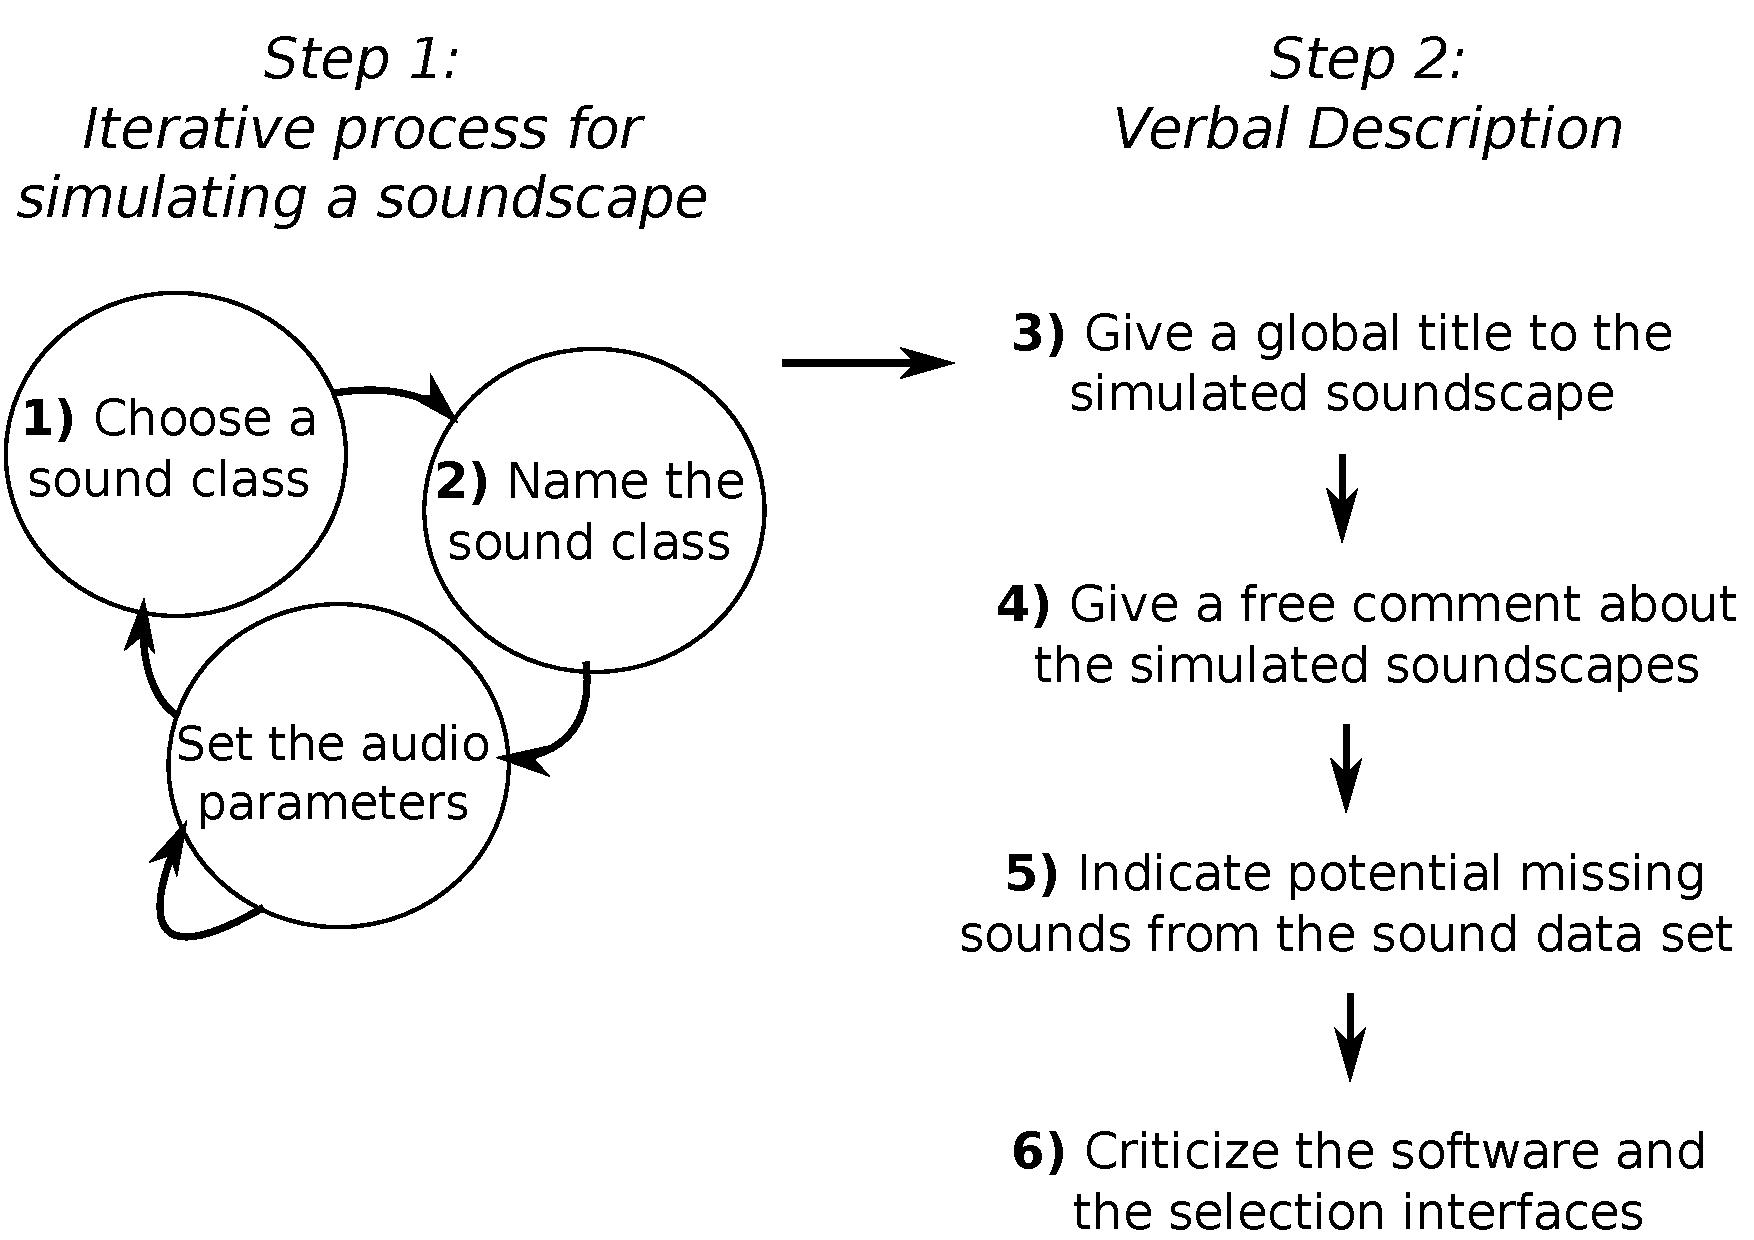
\includegraphics[width=.8\linewidth]{gfx/4}
       \caption{Etape de processus de simulation pour l'analyse sensorielle}\label{fig:etapeSimu}
\end{figure}

\subsection{Paramètres de contrôle}
\label{sec:ch4_param}

Les paramètres de contrôle  permettent au sujet de paramétrer chaque piste. Ils agissent toujours sur tout les samples d'une piste, et jamais sur un en particulier.

Parmi ces paramètres, on retrouve les trois précedemment introduit pour le modèle initial de scène sonore (\cf~section~\ref{sec:ch4_modelParam} et~\ref{sec:ch4_modelForm}), à savoir:

\begin{itemize}
\item \emph{niveau sonore} ($dB$): Pour chaque sample, les niveaux sont tirés aléatoirement à partir d'une distribution normal, paramétré par le sujet en terme de moyenne variance
\item \emph{espacement inter-onset} (seconde): (piste d'événement seulement) comme pour le niveau, les espacements sont tirés aléatoirement à partir d'une distribution normal, paramétré par le sujet en terme de moyenne variance
\item \emph{début et fin} (sec): le sujet fixe le début et la fin de chaque piste.
\end{itemize}

Afin de faciliter la simulation, deux paramètres supplémentaire sont proposés:

\begin{itemize}
\item \emph{fondu par événement} (seconde): (piste d'événement seulement) le sujet fixe une durée de fondu (entrée et sortie), appliqué à chaque sample d'une piste d'événements.
\item \emph{fondu globale} (seconde): le sujet fixe les durées de fondu séparément pour l'entré et la sortie de la piste. Ces fondus s'appliquent ainsi à l'ensemble des samples de la piste.
\end{itemize}

Deux de ces paramètres ne s’appliquent que pour les pistes d'événements (\emph{fondu par événement} et \emph{espacement inter-onset}), les samples des textures étant séquencés sans espacement (\cf~section~\ref{sec:ch4_modelParam})

\subsubsection{Données produites par le processus de simulation}

Ce protocole de simulation peut potentiellement produire un grand nombre de données. Ces dernières sont décrites à la figure~\ref{fig:paradigmeSimu2}.  Nous les résumons dans La liste suivante:

\begin{itemize}
\item Données sémantiques objectives: La banque de données nous permet d'obtenir une information objective quant aux sources sonores présentes dans la scènes. Les données sémantiques objectives sont labels des classes sélectionnées.
\item Données sémantiques subjective: Il s'agit des noms donnés par le sujet 1) à la scène simulée, 2) au classes de sons sélectionnée
\item Données quantitatives issues de la partition: Il s'agit de toutes les données relatives à la partition,\ie~pour chaque piste, le positionnement des samples et les paramètres.
\item Données quantitatives issues du signal: Il s'agit d'indicateur acoustiques extrait du signal,\eg~le niveau sonore globale. Comme nous possédons les samples isolés utilisés pour la synthèse, il est possible de calculer ces descripteurs pour une classe, ou un ensemble de classes en particulier.
\end{itemize}

Le protocole nous permet de caractériser avec précision une scène simulée, sur la base de données sémantique, subjectives ou objectives, ainsi que quantitatives. Considérant l'ensemble des données générés, les potentiels d'analyse sont vaste.

\begin{figure}[bth]
        \myfloatalign
        \includegraphics[width=.8\linewidth]{gfx/2}
       \caption{TODO}\label{fig:paradigmeSimu2}
\end{figure}

\subsection{Interface de sélection aveugle des sons isolés}
\label{sec:ch4_ssf}

Pour limiter l’influence de l’interface sur le sujet, il nous apparaît nécessaire de libérer sa recherche de toute information textuelle. Nous proposons à l'utilisateur une interface graphique lui permettant d’explorer la banque de sons exclusivement à partir de l’écoute.

Visuellement, les classes du dernier niveau (les seules accessibles par le sujet) sont représentés par des cercles et positionnée sur un plan. La disposition des cercles dans l'espace dépend de l’organisation hiérarchique de la base de données: les sous classes appartenant à la même classe sont proches les unes des autres, et ainsi de suite jusqu'à atteindre les classes des niveaux d'abstraction élevés.

La figure~\ref{fig:ssf} présente l'interface pour la banque de données d'événements sonores. Cette organisation visuelle à été pensée afin de:

\begin{enumerate}
\item faciliter le parcours de la banque de données, les sons similaire (au sens des classes) étant proches les uns des autres. L'organisation hiérarchique se fonde sur en effet sur des principes cognitifs. Les classes ont été établies à partir de la littérature traitant des catégories de sources sonore (\cf~section~\ref{xx}).
\item permettre aux sujets de rapidement appréhender toute l'étendue de la banque de données, \ie~l'ensemble des sons disponibles.
\end{enumerate}

Chaque classe possède un son prototype. Ces sons ont été choisis par les expérimentateurs. Lorsqu’on ``\,clique\,'' sur un cercle, le prototype associé à la classe est joué. Le sujet parcours la banque de sons en cliquant sur les cercles.

Cette interface a fait l'objet d'une étude approfondie dont les résultats sont publiés dans \citep{lafay2016JAES}. \gl{Plus sur les résultats ?}

\begin{figure}[bth]
        \myfloatalign
        \includegraphics[width=.8\linewidth]{gfx/SSF}
       \caption{L'interface de sélection aveugle de l'outil de simulation \emph{Simscene}}\label{fig:ssf}
\end{figure}



\subsection{Interface de simulation: l'outil \emph{Simscene}}
\label{sec:ch4_simscene}

\emph{Simscene} est un environnement de travail audio-numérique, supporté par navigateur internet, et développé dans le cadre du projet HOULE\footnote{Pour plus d’informations sur le Projet HOULE voir \url{http://houle.ircam.fr/wordpress/}}. Il permet de simuler des paysages sonores à partir d'un corpus de sons. Il est prévu pour fonctionner via les navigateurs internet \emph{Chrome} et \emph{Firefox}. L'outil a été développé en javascript à l'aide des librairies \emph{web-audio} \footnote{\emph{web-audio}: \Cf~\url{http://www.w3.org/TR/webaudio/}} et \emph{angular.js} \footnote{\emph{angular.js}: \Cf~\url{https://angularjs.org/}}. L'interface de sélection (\cf~section~\ref{sec:ch4_ssf}) a été développée à l'aide de la librairie \emph{D3.js} \citep{d32011}.

\emph{Simscene} et ses fonctionnalités son présentés en détail dans \citep{rossignol2015simscene}, nous résumons ici ses fonctionnalités. 

Le fonctionnement de \emph{Simscene} se rapproche de celui d'un séquenceur audio. Chaque qu’un utilisateur choisit une classe en de son via l'interface de sélection (\cf~section~\ref{sec:ch4_ssf}). Une fois sélectionné, une piste audio, liée à la classe sélectionnée, est créée. L'utilisateur peut alors modifier certaines propriétés de la piste via un groupe de paramètres de contrôle propre à chaque piste audio (\cf~section~\ref{sec:ch4_param}). Des environnements de texte sont prévu afin de permettre à l'utilisateur de 1) nommer chaque piste, 2) donner un titre à la scène simulée et 3) commenter la scène simulée.

L'interface propose un rendu graphique schématisé de la scène en création (\Cf~Figure~\ref{fig:simscene}). La piste est représentée par une bande possédant un axe temporelle. Sur cette bande, chaque sample est représenté par un rectangle. L'espacement entre les rectangle est relatif à l'espacement entre le sample, de même la hauteur des rectangles est relatif au niveau sonore des samples. Dans le cas d'une piste de texture, un unique rectangle apparaît sur toute la longueur de la piste, un son de texture ne pouvant être entrecoupé de silence. Les caractéristiques des rectangles se modifient en fonction des changements de paramètres de la piste.

L'utilisateur a la possibilité à tout moment d'écouter la scène simulée.

\begin{figure}[bth]
        \myfloatalign
        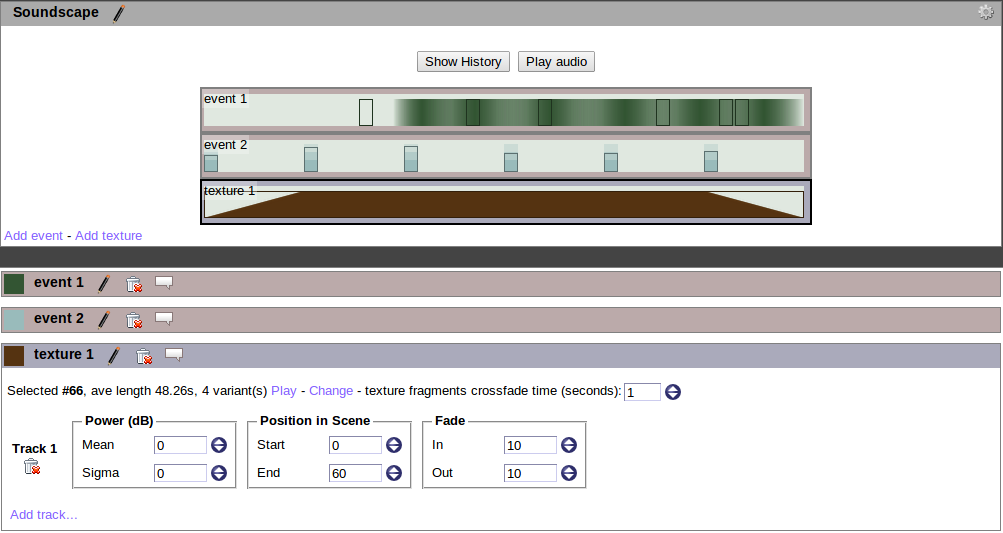
\includegraphics[width=.8\linewidth]{gfx/simscene}
       \caption{L'outil de simulation \emph{Simscene}}\label{fig:simscene}
\end{figure}

L'outil de simulation est accessible via le lien suivant: \url{http://www.irccyn.ec-nantes.fr/~lagrange/
demonstrations/simScene.html}

\section{Du modèle à la simulation dans le cadre de l'analyse automatique}
\label{sec:ch4_modAnaAuto}

%*****************************************
%*****************************************
%*****************************************
%*****************************************
%*****************************************
